\documentclass[crop=false,fleqn]{standalone}
\usepackage{../../../globle-preamble}

\begin{document}
    \textbf{Express the Volume $V$ of a cube as a function of the area $A$ of its base.}

    \begin{center}
        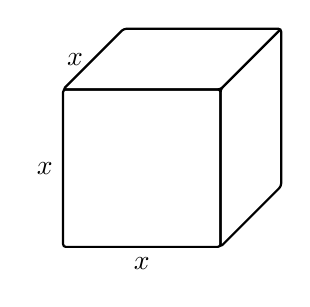
\begin{tikzpicture}
            \def\cubex{2}
            \def\cubey{2}
            \def\cubez{2}

            \draw[thick,rounded corners=1pt]
                (0,0,0) -- ++(-\cubex,0,0) -- node[left]{$x$} ++(0,-\cubey,0)
                -- node[below]{$x$} ++(\cubex,0,0) -- cycle;
            \draw[thick,rounded corners=1pt]
                (0,0,0) -- ++(0,0,-\cubez) -- ++(0,-\cubey,0) -- ++(0,0,\cubez)
                -- cycle;
            \draw[thick,rounded corners=1pt]
                (0,0,0) -- ++(-\cubex,0,0) -- node[left]{$x$} ++(0,0,-\cubez)
                -- ++(\cubex,0,0) -- cycle;
        \end{tikzpicture}
    \end{center}

    Let $x$ be the each side of cube

    \begin{equation*}
        \begin{split}
            \text{Volume of cube} = V &= x\times x\times x \\
                                    &= x^3 \\
            \\
            \text{Area of base} = A &= x \times x \\
                                    &= x^2 \\
                        \implies x &= \sqrt{A}
        \end{split}
    \end{equation*}

    Putting $x=\sqrt{A}$ in $V=x^3$:

    \begin{equation*}
        \begin{split}
            V &= \left(\sqrt{A}\right)^3 \\
            &= A^{3/2}
        \end{split}
    \end{equation*}

    The above relation expresses the volume $V$ of a cube as a function of the area $A$ of its base.
\end{document}